\section{Early Assessment and Budgeted Search}
\label{app:semantic-budget}
An early semantic assessment asks whether a proposed interpretation is likely to preserve the source obligations and assumptions. Its prediction can guide which candidate receives the next formalization attempt. Research Preference Models motivate assessing candidates before costly execution~\cite{foster2026rpm}; reusable algorithmic structure provides a reason to expect earlier experience to help the search~\cite{e28030332}. Verification and human review then assess the resulting artifacts and their scope.

\subsection{Semantic Prediction and Its Geometry}
The workbench supplies the comparisons and forecasts in Table~\ref{tab:semantic-comparisons}~\cite{scpCheckpoint}. Automatic use of their predictions to admit attempts and rank search branches is a proposed extension. The later SNG reconstruction supplied 66 preselected entries in its $K^{+}$ input and used that set throughout. Section~\ref{sec:fidelity} describes the separate source and contract reviews.

\begin{table}[!htbp]
\caption{Comparison inputs and outputs in the inspected implementation.}
\label{tab:semantic-comparisons}
\centering\small
\begin{tabular}{@{}p{.20\linewidth}p{.43\linewidth}p{.31\linewidth}@{}}
\hline
Mechanism & Inputs & Output and use \\
\hline
Rule retrieval & Task query; rule trigger and principle & Lexical cosine distance; selects related guidance. \\
Contract comparison & Features of assumptions and guarantees after architecture assessment & Cosine distance; supports review of contract differences. \\
Model forecast & Reviewed learning material, declared task, and available feedback & Model belief score and explanation for the next application. \\
\hline
\end{tabular}
\end{table}

For rule retrieval, $x$ counts words and symbols in the task query and $y$ those in a rule's trigger and principle. Nonzero vectors satisfy the configured comparison when
\begin{equation}
d_{\cos}(x,y)=1-\frac{x\cdot y}{\|x\|\|y\|}\leq\epsilon.
\label{eq:retrieval-distance}
\end{equation}
The retrieval default is $\epsilon=0.1$, with allowed values in $[0,0.3]$. Contract comparison uses features of assumptions and guarantees after architecture checking. These representations approximate similarity: counting words and symbols gives $a\leq b$ and $b\leq a$ the same representation. A model assessment can examine the relation and explain uncertainty. A distance limit corresponds to an angle $\theta_{\max}=\arccos(1-\epsilon_{\max})$ around the reference direction.

Figure~\ref{fig:semantic-cone} retains the reference, candidate directions, and applicability boundary illustrated by Tahat et al.~\cite[slide~12]{tahat2026dascslides}. Green and check marks denote a favorable prediction that sends a candidate to formal assurance within the remaining budget. Crosses identify illustrative candidates for refinement or review. The construction extends to any specification language for which paired requirements, candidate representations, and suitable checks are defined; the engineering cases here use SysML/GUMBO. Forecast calibration is a subject for future evaluation.

\begin{figure}[!htbp]
\centering
% Vector redraw of Tahat et al., slide 12. Marks show illustrative predictions.
\begingroup
\hyphenpenalty=10000
\begin{tikzpicture}[
 x=1cm,y=1cm,font=\sffamily\fontsize{8.5}{10}\selectfont,
 arrow/.style={-{Stealth[length=1.8mm,width=1.3mm]},line width=.8pt},
 note/.style={align=center,fill=white,inner sep=3pt},
 good/.style={text=scpGreen,font=\sffamily\bfseries\fontsize{12}{13}\selectfont},
 bad/.style={text=scpRed,font=\sffamily\bfseries\fontsize{12}{13}\selectfont}
]
\path[fill=scpRedFill] (.35,0) --
  plot[domain=.35:11.65,samples=90] (\x,{3.6*exp(-((\x-6)^2)/8)}) -- (11.65,0) -- cycle;
\path[fill=scpGreenFill] (6,0) --
  plot[domain=3.65:8.35,samples=50] (\x,{3.6*exp(-((\x-6)^2)/8)}) -- cycle;
\draw[arrow,draw=black!50] (.15,0) -- (12.1,0);
\node[rotate=90,align=center] at (-.30,1.95)
  {Illustrative predicted suitability};
\node[align=center] at (6,-.44)
  {Candidate representations for a chosen specification language};
\draw[black!70,line width=1.2pt,domain=.35:11.65,samples=90]
  plot (\x,{3.6*exp(-((\x-6)^2)/8)});
\foreach \x/\lab in {4.9/{\mathbf v'_1},7.1/{\mathbf v_1},4.15/{\mathbf v'_2},7.85/{\mathbf v_2}}{
  \pgfmathsetmacro{\yy}{3.6*exp(-((\x-6)^2)/8)}
  \draw[arrow,black!40] (6,0) -- (\x,\yy);
  \fill[black!80] (\x,\yy) circle (2pt);
  \node[above] at (\x,\yy+.09) {$\lab$};
}
\draw[arrow,scpBlue,line width=2pt] (6,0) -- (6,4.45);
\node[note,text=scpBlue] at (6,4.76)
  {\textbf{Reviewed reference $g$}\\English requirement + formal specification};
\foreach \x in {3.65,8.35}{
  \draw[scpRed,line width=1pt] (6,0) -- (\x,1.806);
  \fill[scpRed] (\x,1.806) circle (2.5pt);
}
\draw[scpRed,dashed,line width=.8pt] (3.65,1.806) -- (2.12,2.982);
\draw[scpRed,dashed,line width=.8pt] (8.35,1.806) -- (9.88,2.982);
\draw[arrow,scpRed] (6,1.05) arc[start angle=90,end angle=37.55,radius=1.05];
\node[note,inner sep=1pt,text=scpRed] at (6.62,1.23) {$\theta_{\max}$};
\node[note,text=scpRed,inner sep=2pt] at (9.55,1.85)
  {$d_{\cos}=\epsilon_{\max}$};
\node[good] at (5.03,2.38) {$\checkmark$};
\node[good] at (6.92,2.38) {$\checkmark$};
\node[bad] at (2.82,.57) {$\times$};
\node[bad] at (9.18,.57) {$\times$};
\node[note,text=scpGreen] at (6,.58)
  {\textbf{Favorable prediction}\\Proceed to formal assurance};
\node[note,text=scpRed,inner sep=2pt] at (1.85,1.08) {Refine or\\request review};
\node[note,text=scpRed,inner sep=2pt] at (10.2,1.08) {Refine or\\request review};
\draw[arrow,draw=orange!85!black] (8.2,4.08) to[out=-12,in=120] (10.35,2.87);
\node[note,inner sep=2pt,text=orange!85!black] at (10.1,3.98) {Broaden applicability};
\draw[arrow,draw=scpRed] (10.65,3.52) to[out=140,in=-10] (8.2,4.48);
\node[note,inner sep=2pt,text=scpRed] at (10.1,4.65) {Narrow applicability};
\node[draw=scpBlue,fill=scpBlueFill,rounded corners=2pt,
  text width=9.0cm,align=center,inner sep=5pt] at (6,5.67)
  {\textbf{Refine the rule and its conditions for use}\\
   Predictions guide the next attempt within allowance $B$.};
\end{tikzpicture}
\endgroup

\caption{Semantic prediction around a reviewed reference, redrawn from Tahat et al.~\cite[slide~12]{tahat2026dascslides}. Green and check marks indicate favorable predictions: proceed to formal assurance. Red and crosses indicate refinement or review. Positions, heights, and marks are illustrative. The geometry applies to a chosen representation in any specification language; formal checks and human decisions establish the accepted scope.}
\Description{A blue reference direction for reviewed English and a formal specification lies at the center of a bell-shaped illustration. Symmetric candidate directions lie inside and outside a distance boundary. Green checks predict suitability for the next assurance phase; red crosses request refinement or review. Arrows broaden or narrow applicability.}
\label{fig:semantic-cone}
\end{figure}

\subsection{Rule Application and Budgeted Search}
Changing $\epsilon$ broadens or narrows the similarity comparison. Revising a rule changes its conditions and procedure. Each application retains the selected version and supporting evidence.

Figure~\ref{fig:budget-tree} follows Tahat et al.~\cite[slide~7]{tahat2026dascslides} from requirements through formalization and placement to code and proof. An incorrect assumption or placement can affect several downstream artifacts. Checking an earlier choice can reveal a repair before those descendants are generated. The displayed branch counts illustrate this dependency.

\begin{figure}[!htbp]
\centering
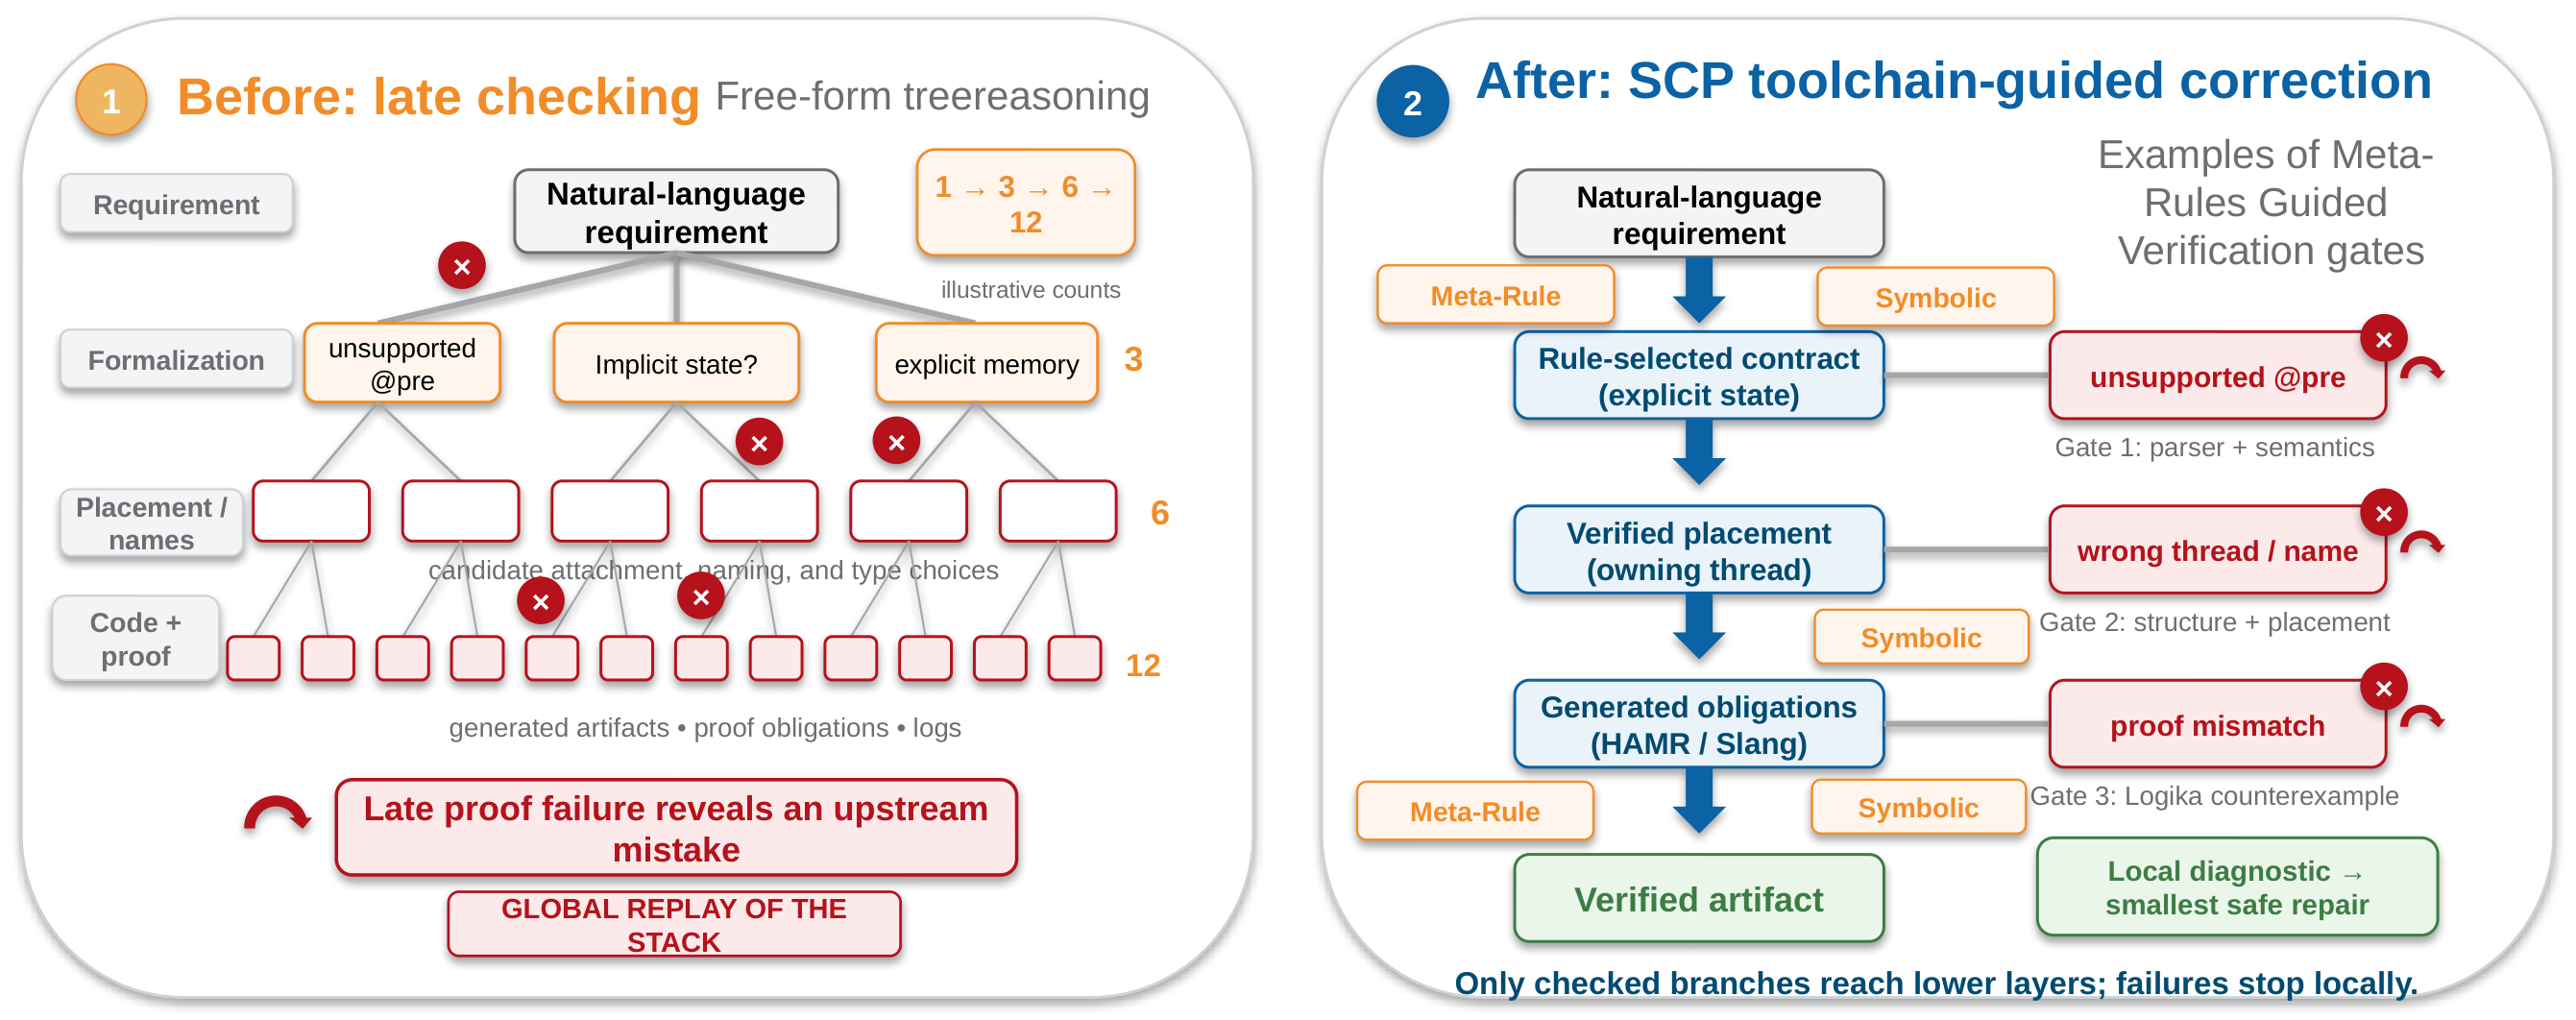
\includegraphics[width=.90\linewidth]{assets/dasc-branching-snapshot.png}
\caption{Late checking and local repair, cropped from the presentation by Tahat et al.~\cite{tahat2026dascslides}. The left panel illustrates how an early choice can multiply downstream artifacts before a failure is detected. The right panel shows checks on formalization, placement, and proof that return diagnostics at the failing stage. The branch counts are illustrative.}
\Description{The left panel is a branching tree from a requirement through formalization and placement choices to code and proof artifacts. The right panel shows a candidate contract, its placement, and proof obligations, with local repair feedback at each of three checks.}
\label{fig:branching-motivation}
\end{figure}

\begin{figure}[!htbp]
\centering
% Native vector redraw of the branching and local-check concept in Tahat et al., slide 7.
\begingroup
\hyphenpenalty=10000
\begin{tikzpicture}[
 x=1cm,y=1cm,font=\sffamily\fontsize{8.3}{9.7}\selectfont,
 edge/.style={draw=black!65,line width=.65pt},
 flow/.style={-{Stealth[length=1.6mm,width=1.2mm]},line width=.75pt},
 branch/.style={draw=black!65,fill=white,rounded corners=1pt,
   minimum width=.27cm,minimum height=.22cm,inner sep=0pt},
 stage/.style={draw=black!65,fill=scpBlueFill,rounded corners=2pt,
   align=center,text width=2.30cm,minimum height=.67cm,inner sep=4pt},
 repair/.style={draw=black!65,dashed,fill=scpGrayFill,rounded corners=2pt,
   align=center,text width=1.25cm,minimum height=.63cm,inner sep=3pt}
]
\path[draw=black!50,rounded corners=2pt] (-.2,.10) rectangle (7.14,5.40);
\path[draw=black!50,rounded corners=2pt] (7.30,.10) rectangle (13.05,5.40);
\node[font=\sffamily\bfseries\fontsize{9}{10.4}\selectfont] at (3.4,5.10)
  {Search alternatives};
\node[font=\sffamily\bfseries\fontsize{9}{10.4}\selectfont] at (10.17,5.10)
  {Check before expanding};
\node[align=left,text width=1.3cm,anchor=west] at (-.08,4.35) {Input};
\node[align=left,text width=1.3cm,anchor=west] at (-.08,3.20) {Formalize};
\node[align=left,text width=1.3cm,anchor=west] at (-.08,2.05) {Placement / names};
\node[align=left,text width=1.3cm,anchor=west] at (-.08,.90) {Code / proofs};
\node[branch] (root) at (4,4.35) {};
\foreach \x [count=\i] in {2.2,4.0,5.8}{
  \node[branch] (f\i) at (\x,3.20) {};
  \draw[edge] (root) -- (f\i);
}
\foreach \x [count=\i] in {1.75,2.65,3.55,4.45,5.35,6.25}{
  \node[branch] (p\i) at (\x,2.05) {};
  \pgfmathtruncatemacro{\parent}{ceil(\i/2)}
  \draw[edge] (f\parent) -- (p\i);
  \node[branch] (l\i) at (\x-.225,.90) {};
  \node[branch] (r\i) at (\x+.225,.90) {};
  \draw[edge] (p\i) -- (l\i);
  \draw[edge] (p\i) -- (r\i);
}
\foreach \y/\count in {4.35/1,3.20/3,2.05/6,.90/12}
  \node[font=\bfseries] at (6.88,\y) {\count};
\node[font=\sffamily\fontsize{8}{9.2}\selectfont] at (4,.40) {Illustrative counts};
\node[stage,fill=scpGrayFill] (req) at (9.08,4.35) {Requirements};
\node[stage] (formal) at (9.08,3.20) {Formalize + check};
\node[stage] (place) at (9.08,2.05) {Placement + check};
\node[stage] (proof) at (9.08,.90) {Code/proof + check};
\draw[flow] (req) -- (formal);
\draw[flow] (formal) -- (place);
\draw[flow] (place) -- (proof);
\foreach \stageName/\stageY in {formal/3.20,place/2.05,proof/.90}{
  \node[repair] (fix-\stageName) at (11.86,\stageY) {Local repair};
  \draw[flow,dashed] (\stageName.east) -- (fix-\stageName.west);
  \draw[flow,dashed] (fix-\stageName.south) to[out=-100,in=-80,looseness=.65] (\stageName.south east);
}
\node[draw=black!55,fill=scpGrayFill,rounded corners=2pt,align=center,
  text width=12.6cm,inner sep=5pt] at (6.42,-.62)
  {\textbf{Approved allowance $B$ covers the continuing search.}\\[3pt]
   Retain prior consumption; further attempts require current authority and remaining allowance.};
\end{tikzpicture}
\endgroup

\caption{Illustrative search and local repair, redrawn from Tahat et al.~\cite[slide~7]{tahat2026dascslides}. The $1\rightarrow3\rightarrow6\rightarrow12$ expansion shows possible branching. Checks can stop an unsuitable choice and return diagnostics to the stage that produced it. These counts describe the illustration; the experiments report their actual attempts and consumption separately.}
\Description{The left tree grows from one requirement to three formalizations, six placement choices, and twelve code or proof branches. The right path checks formalization, placement, and proof choices as they arise, with local repair loops. One approved allowance covers earlier and future attempts.}
\label{fig:budget-tree}
\end{figure}

\paragraph{Proposed agreement and cost prediction}
For a requirement and candidate under stated premises, an agreement model could learn from human review outcomes, using the on-demand forecast and contract-feature similarity as inputs. A cost model could estimate incremental wall time and model tokens from attempts with comparable artifact sizes, check plans, and tool versions. Candidate ordering would favor likely agreement within the remaining time and token allowance. Estimates with sparse supporting records would carry uncertainty and could trigger review. Linking predictions to observed costs and review outcomes would let us evaluate calibration and saved effort.

Further attempts require current authority, an unexpired deadline, and available allowance after recorded consumption and outstanding reservations. Unresolved usage blocks further model calls. A stopped branch retains its attempted artifacts, diagnostics, and charges. An implementation repair can continue within current authority; a change to requirements, assumptions, scope, or limits returns to human review. A current failed use of the same rule and learning plan can supply feedback for rule revision. An authorized extension preserves earlier consumption across the continuing campaign.
